    %%%%%%%%%%%%%%%%%%%%%%%%%%%%%%%%%%%%%%%%%%%%%%%%%%%%%%%%%%%%
%%  This Beamer template was created by Cameron Bracken.
%%  Anyone can freely use or modify it for any purpose
%%  without attribution.
%%
%%  Last Modified: January 9, 2009
%%

\documentclass[xcolor=x11names,compress]{beamer}

%% General document %%%%%%%%%%%%%%%%%%%%%%%%%%%%%%%%%%
\usepackage{graphicx}
\usepackage{tikz}
\usepackage{xcolor}
\usetikzlibrary{decorations.fractals, arrows, shapes, calc}
%%%%%%%%%%%%%%%%%%%%%%%%%%%%%%%%%%%%%%%%%%%%%%%%%%%%%%


%% Beamer Layout %%%%%%%%%%%%%%%%%%%%%%%%%%%%%%%%%%
\useoutertheme[subsection=false,shadow]{miniframes}
\useinnertheme{default}
\usefonttheme{serif}
\usepackage{palatino}

\setbeamerfont{title like}{shape=\scshape}
\setbeamerfont{frametitle}{shape=\scshape}

\setbeamercolor*{lower separation line head}{bg=DeepSkyBlue4}
\setbeamercolor*{normal text}{fg=black,bg=white}
\setbeamercolor*{alerted text}{fg=red}
\setbeamercolor*{example text}{fg=black}
\setbeamercolor*{structure}{fg=black}

\setbeamercolor*{palette tertiary}{fg=black,bg=black!10}
\setbeamercolor*{palette quaternary}{fg=black,bg=black!10}

\renewcommand{\(}{\begin{columns}}
\renewcommand{\)}{\end{columns}}
\newcommand{\<}[1]{\begin{column}{#1}}
\renewcommand{\>}{\end{column}}
\tikzset{onslide/.code args={<#1>#2}{%
  \only<#1>{\pgfkeysalso{#2}} % \pgfkeysalso doesn't change the path
}}  
%%%%%%%%%%%%%%%%%%%%%%%%%%%%%%%%%%%%%%%%%%%%%%%%%%




\begin{document}


%%%%%%%%%%%%%%%%%%%%%%%%%%%%%%%%%%%%%%%%%%%%%%%%%%%%%%
%%%%%%%%%%%%%%%%%%%%%%%%%%%%%%%%%%%%%%%%%%%%%%%%%%%%%%


\begin{frame}
\title{\huge Time-optimised Route Planning for Electric Vehicles}
%\subtitle{SUBTITLE}
\author{
 Simon Buus Jensen,\\
 Andreas Berre Eriksen,\\
 Mikkel Alexander Madsen,\\
 Mathias Meldgaard Andersen\\
}
\titlepage
\end{frame}

\begin{frame}{Table of Contents}
\tableofcontents
\end{frame}

\section{\scshape Introduction}
\subsection{Motivation}
\begin{frame}{Motivation}
\begin{itemize}
\item Why is route planning for EVs an interesting problem?
\end{itemize}
\begin{figure}[h!]
  \centering
  Plug-in Vehicle production
    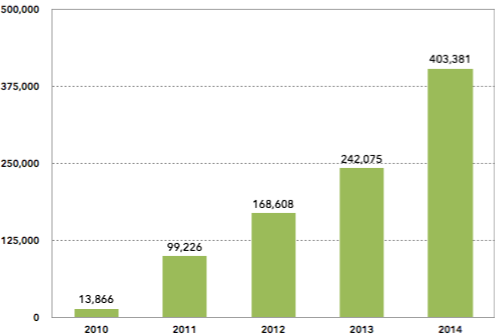
\includegraphics[height=0.5\textwidth]{images/forecast}
  
      \tiny Credit: IHS automotive
\end{figure}
\end{frame}

\begin{frame}{Motivation}
\begin{itemize}
\item Why is route planning for EVs an interesting problem?
\end{itemize}
\begin{figure}[h!]
  \centering
  Fast-charging stations worldwide
    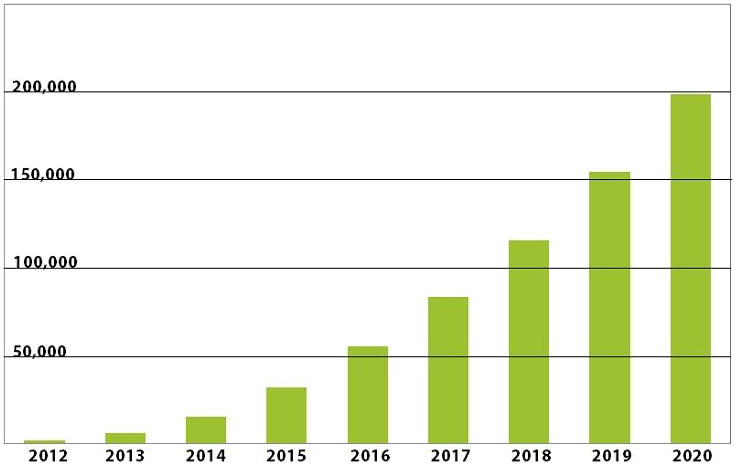
\includegraphics[height=0.5\textwidth]{images/forecast2}
  
      \tiny Credit: IHS automotive
\end{figure}
\end{frame}

\subsection{Greedy Heuristics Algorithm}
\todo[inline]{introductory text}

\subsubsection*{Idea outline}
The idea of the approach taken in this section, is using Dijkstra's algorithm for finding the shortest path with $\frac{distance}{speed}$ as the weight of an edge. The problem then becomes, which speed must we use in the interval of $v_{min}$ and $v_{max}$. As argued previously, the optimal speed to drive can only be found by iterating over all possibilities which is a combinatorial optimization problem, and it is NP-Hard. Thus we introduce a heuristic, which promotes local optimal choices. This gives a fast path, but this might not be drivable, if there are not any charge stations on this path, thus we will need to figure out how to incorporate this.\\

We will now analyse how the weight can be found, specifically the speed. The time spent passing an edge $e = (u_1, u_2)$ in the road network, is given by the following equation:
\begin{equation*}
\begin{aligned}
 & T(v,(u_1, u_2)) = \frac{D((u_1, u_2))}{v} + \frac{R_{CO}(v) * D((u_1, u_2)) - B_{cur}}{Best_{CH}(u_1)}
\end{aligned}
\end{equation*}\label{eq:drivingAndCharging}

where $v$ is the speed of the vehicle, $D(u_1, u_2)$ is the distance between vertices $u_1$ and $u_2$, $R_{CO}(v)$ is the consumption rate of the vehicle at the speed $v$, $B_{cur}$ is the current battery capacity of the vehicle and $Best_{CH}(u_1)$ is the charge rate of the best charge station previous to $u_1$ or the charge rate ofs $u_1$.The above equation yields a function on the form: $av^2 + bv + c$, due to the fact that $R_{CO}(v)$ is a quadratic function. $a$ , $b$ and $c$ are some constants which are given by the instance of the vehicle. 
Represented in a Cartesian coordinate system, $T(v,(u_1, u_2)))$ is a parabola, as can be seen in Figure \ref{fig:graph}. On the x-axis is the speed of the vehicle and on the y-axis is the time spent. The turning point of the graph represents the optimal speed to drive at for the given edge, denoted as $v_{opt}(e)$. The point is easily calculated by finding a tangent line with a slope of $0$. If $v_{opt}(e)$ is smaller than $v_{min}(e)$, then $v_{min}(e)$ defines the optimal speed for the edge. Similarly if $v_{opt}(e)$ is larger than $v_{max}(e)$, $v_{max}(e)$ defines the optimal speed for the edge.\\


\begin{figure}[!htb]
\label{fig:graph}
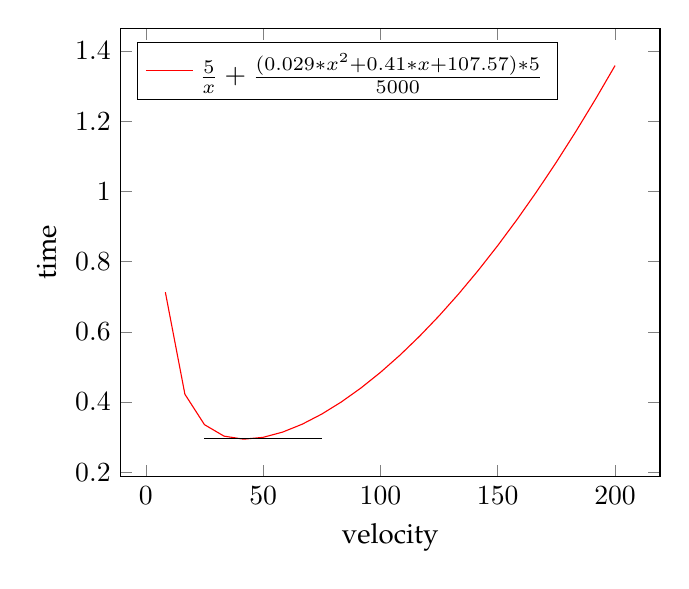
\begin{tikzpicture}
\begin{axis}[xlabel=velocity, ylabel=time,legend style={legend pos=north west}]
\addplot[draw=red,domain=0:200]{(5/x)+(((0.0286*x^2 + 0.4096*x + 107.57)*5)/5000)};
\addlegendentry{$\frac{5}{x}+\frac{(0.029*x^2 + 0.41*x + 107.57)*5}{5000}$}

\addplot[draw=black,domain=25:75]{0.295};
% \addplot[mark=*, domain=25:75] coordinates {(37,295)};
\end{axis}
\end{tikzpicture}% 
\caption{In this instance of $T(v,(u_1, u_2))$, going from $u_1$ to $u_2$, we have a distance of $5 \si{\km}$ and a charge speed of $5 \si{\kW}$ on $u_1$. The optimal speed in this case is $42.12\si{\miles\per\hour}$, which takes roughly 7 minutes to drive}
\end{figure}





While the algorithm progresses through the graph, it need to store a subset of the charge stations on the current path. At every reached charge station, we record the possible energy$B_{possible}$ we can add to the system, defined by $B_{cap}-B_{cur}$ and the charge rate of the station as a tuple: $(B_{possible}, R_{CH}(vertex))$.\\
We maintain a subset of tuples on every vertex by using a list of tuples only with $B_{possible}$ above 0. This will of course always be the case when we reach a charge station, but as we progress through the graph and some distance is being traveled, the possible energy at each previous charge station decreses. The first tuple in the list will always be the the charge station with the best charge rate. A tuple is removed either when $B_{possible}$ hit 0, or when new tuple, with a higher charge rate is found. We make sure to store the best charge station at position 0 in the list, by remove every tuple between the first and second best charge rate in the list.\\

Using this we can define a fastest path algorithm in the following way: \\

\begin{algorithmic}
\Function{GreedyHeuristic}{$RN,s,t,EV$}
	\ForAll{$v \in RN.V$} 
		\State $v.time = \infty$
		\State $v.predecessor = NIL$
		\State $v.preCS = NIL$
		\State $v.B_{cur} = NIL$
	\EndFor
	\State $s.time = 0$
	\State $s.B_{cur} = EV.B_{cur}$

	\State $Q = PriorityQueue$
	\State $INSERT(Q, (s.time, s))$	
	\While{$Q \neq \emptyset$} 
		\State $u = extract-min(Q)$
		\ForAll{each vertex $v \in RN.adj(u)$} 
			\State $time,preCS,B_{cur},energy = travel\_time(RN, u, EV)$
			\If{$v.time > u.time + time$} 
				\State $v.time = u.time + time$
				\State $v.predecessor = u$
				\State $v.B_{cur} = B_{cur}$
				\State $v.preCS = preCS$
				\State $insert(Q, (v.time, v))$	
			\EndIf

		\EndFor
	\EndWhile
	\State \Return $t.time, t.path$
\EndFunction
\end{algorithmic}\label{alg:fastest_path}


\section{Optimal solution to a path}
\subsection{Modeling of the physical system}
\begin{frame}{Physical system}
Modeling the physical system, of an EV and a path.
\begin{figure}[!htb]
\centering
    \begin{tikzpicture}[shorten >=1pt,node distance=2.5cm,>=stealth',thick]
        \node[state] (1) {$u_1$};
        \node[state] (2) [right of=1] {$u_2$};
        \node[] (dots) [right of=2] {$\dots$};
        \node[state] (n) [right of=dots] {$u_n$};
        \node[state,draw=none] (d1) [right of=n] {};
        \draw [->] (1) to[right] node[auto] {$e_1$} (2);
        \draw [->] (2) to[right] node[auto] {$e_2$} (dots);
        \draw [->] (dots) to[right] node[auto] {$e_{n-1}$} (n);
        %\draw [->] (n) to[right] node[auto] {$e_n$} (d1);
    \end{tikzpicture}
\end{figure} 
\begin{itemize}
\item Path
\begin{itemize}
\item[+] Charging stations, with charging rate ($R_{CH}(u_i)$)
\item[+] Road segments, with speed limit ($v_{min}(e_i)$, $v_{max}(e_i)$) and distance ($D(e_i)$) 
\end{itemize}
\item EV
\begin{itemize}
\item[+] Driving consumes energy accordingly to the speed of the EV, defined by: ($R_{CO}(e_i)$)
\item[+] Further two constants from the EV are important to model, namely, battery capacity ($B_{max}$) and initial battery ($B_{cur}$)
\end{itemize}
\end{itemize} 
\end{frame}
\subsection{Optimisation problem}
\begin{frame}{optimisation}
Formulating a optimisation problem, which when solved will yield a optimal solution. 
\begin{itemize}
\item Objective: Move from $u_1$ to $u_n$ using minimum time . 
\begin{itemize}
\item[+] Time can be used driving or charging. 
\begin{itemize}
\item[-] $\text{min: } \sum_{i=1}^{n-1} \left(\frac{D(e_i)}{v_{e_i}} + CT_{u_i} \right)$
\end{itemize}
\end{itemize}
\item Physical constraints:
\begin{itemize}
\item[+] Each edge must be driven at a speed within the speed limit:\begin{itemize}
\item [-] $\forall_{i\in1 \dots n-1 }:\;v_{min}(e_i) \leq v_{e_i} \leq v_{max}(e_i)$
\end{itemize}
\item[+] Time can only be positive.\begin{itemize}
\item [-] $\forall_{i\in1 \dots n }:\; 0 \leq CT_{u_i} $
\end{itemize}

\item[+] The energy is the battery must alway be between 0 and $B_{max}$
\end{itemize}
\end{itemize} 
\end{frame}
\begin{frame}{battery constraint}
The battery constraint of the optimisation problem can be split into two parts
\begin{itemize}
\item No road segment can be passed without having the required energy
\item No overcharging at any charging station. 
\end{itemize}
Energy can be..
\begin{itemize}
\item Spend: $\forall_{i\in1 \dots n-1 }:\; ES(e_i) = D(e_i) \times R_{CO}(v_{e_i})$
\item Acuried: $\forall_{i\in1 \dots n }:\; EA(u_i) = R_{CH}(u_i) \times CT_{u_i}$
\item Already in the battery: $B_{cur}$
\end{itemize}
\end{frame}
\begin{frame}{battery constraint}
No road segment can be passed without having the required energy 
\begin{figure}[!htb]
\centering
    \begin{tikzpicture}[shorten >=1pt,node distance=2.5cm,>=stealth',thick]
        \node[state] (1) {$u_1$};
        \node[state] (2) [right of=1] {$u_2$};
        \node[] (dots) [right of=2] {$\dots$};
        \node[state] (n) [right of=dots] {$u_n$};
        \node[state,draw=none] (d1) [right of=n] {};
        \draw [->] (1) to[right] node[auto] {$e_1$} (2);
        \draw [->] (2) to[right] node[auto] {$e_2$} (dots);
        \draw [->] (dots) to[right] node[auto] {$e_{n-1}$} (n);
        %\draw [->] (n) to[right] node[auto] {$e_n$} (d1);
        \draw[decorate,decoration={brace,amplitude=5pt,mirror}] 
    (-0.5,-0.5) coordinate (1) -- (2,-0.5) coordinate (2);
    \node at (0.8,-1.0){$i=1$};
     \draw[decorate,decoration={brace,amplitude=5pt,mirror}] 
    (-0.5,-1.5) coordinate (1) -- (4.5,-1.5) coordinate (2);
    \node at (2.1,-2.0){$i=2$};
    \draw [dashed] (2.5,-2.5) -- (4,-2.5);
     \draw[decorate,decoration={brace,amplitude=5pt,mirror}] 
    (-0.5,-3.5) coordinate (1) -- (7,-3.5) coordinate (2);
    \node at (3.4,-4.0){$i=n-1$};

    \end{tikzpicture}
\end{figure} 
\begin{itemize}
\item $\forall_{i\in1 \dots n-1 }:\;0 \leq B_{cur} + \sum_{j=1}^{i} EA(u_j) - \sum_{j=1}^{i} ES(e_j) \leq B_{max}$
\end{itemize}
\end{frame}

\begin{frame}{battery constraint}
No overcharging at any charging station.
\begin{figure}[!htb]
\centering
    \begin{tikzpicture}[shorten >=1pt,node distance=2.5cm,>=stealth',thick]
        \node[state] (1) {$u_1$};
        \node[state] (2) [right of=1] {$u_2$};
        \node[] (dots) [right of=2] {$\dots$};
        \node[state] (n) [right of=dots] {$u_n$};
        \node[state,draw=none] (d1) [right of=n] {};
        \draw [->] (1) to[right] node[auto] {$e_1$} (2);
        \draw [->] (2) to[right] node[auto] {$e_2$} (dots);
        \draw [->] (dots) to[right] node[auto] {$e_{n-1}$} (n);
        %\draw [->] (n) to[right] node[auto] {$e_n$} (d1);
        \draw[decorate,decoration={brace,amplitude=5pt,mirror}] 
    (-0.5,-0.5) coordinate (1) -- (3,-0.5) coordinate (2);
    \node at (1.3,-1.0){$i=1$};
     \draw[decorate,decoration={brace,amplitude=5pt,mirror}] 
    (-0.5,-1.5) coordinate (1) -- (5.5,-1.5) coordinate (2);
    \node at (2.6,-2.0){$i=2$};
    \draw [dashed] (3,-2.5) -- (6.5,-2.5);
     \draw[decorate,decoration={brace,amplitude=5pt,mirror}] 
    (-0.5,-3.5) coordinate (1) -- (8,-3.5) coordinate (2);
    \node at (3.9,-4.0){$i=n-1$};

    \end{tikzpicture}
\end{figure} 
\begin{itemize}
\item $\forall_{i\in1 \dots n-1}:\;0 \leq B_{cur} + \sum_{j=1}^{i+1} EA(u_j) - \sum_{j=1}^{i} ES(e_j) \leq B_{max}$
\end{itemize}
\end{frame}

\subsection{Linear programming}
\begin{frame}{Linear programming}
NP-complete problem.

Linearization and linear programming for approximate solution. 

Two functions of the optimisation problem are non linear functions. 
\begin{itemize}
\item Consumption rate ($R_{CO}(v_{e_i})$)
\item Driving time ($\frac{D(e_i)}{v_{e_i}}$)
\end{itemize}
\end{frame}


\begin{frame}{linearization example}
Function for energy consumption before linearization. $R_{CO}(v)=0.019*x^2 - 0.770*x + 184.4$
\begin{figure}[!htb]
\label{fig:graph}
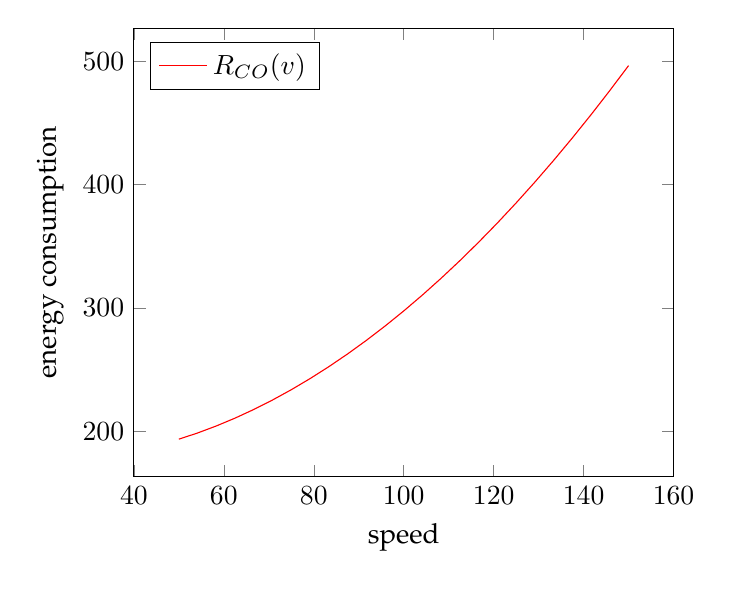
\begin{tikzpicture}
\begin{axis}[xlabel=speed, ylabel=energy consumption,legend style={legend pos=north west}]
\addplot[draw=red,domain=50:150]{(0.019*x^2 - 0.770*x + 184.49) };
\addlegendentry{$R_{CO}(v)$}

% \addplot[mark=*, domain=25:75] coordinates {(37,295)};
\end{axis}
\end{tikzpicture}% 

\label{fig:graph}
\end{figure}
\end{frame}

\begin{frame}{linearization example}
Function for energy consumption after linearization. $R_{CO}(v)=0.019*x^2 - 0.770*x + 184.4$
\begin{figure}[!htb]
\label{fig:graph}
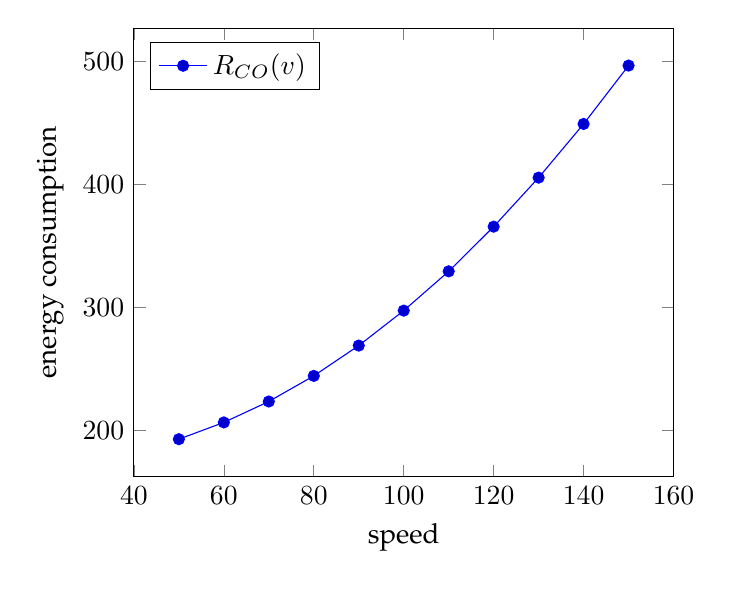
\begin{tikzpicture}
\begin{axis}[xlabel=speed, ylabel=energy consumption,legend style={legend pos=north west}]
\addplot coordinates { (50,193) (60,206.6) (70,223.6) (80,244.4) (90,269) (100,297.4) (110,329.3) (120,365.6) (130,405.4) (140, 449) (150,496.4) }; \addlegendentry{$R_{CO}(v)$ }

% \addplot[mark=*, domain=25:75] coordinates {(37,295)};
\end{axis}
\end{tikzpicture}% 

\label{fig:graph}
\end{figure}
\begin{itemize}
\item For all linear function their slope and the y-intercept is precomputed. 
\item For every edge in the path exactly one line segment needs to be chosen. Thus a binary matrix i introduced of size $n \times m$, where $n=$edges in the path and $m=$linear pieces of each line. 
\end{itemize}
\end{frame}
\begin{frame}{linearization example}
\begin{itemize}
\item For all linear function their slope and the y-intercept is precomputed. 
\item For every edge in the path exactly one line segment needs to be chosen. Thus a binary matrix i introduced of size $n \times m$, where $n=$edges in the path and $m=$linear pieces of each line. 
\end{itemize}
\end{frame}




\section{\scshape Experiments}
\subsection{this shit}
\begin{frame}
  \frametitle{Experiments}
  \begin{itemize}
  	\item Why experiments?
  	\item Map data (Open Street Maps)
  	\item Conversion to road network
  \end{itemize}
\end{frame}

\begin{frame}
  \frametitle{Experiments: The Setup} 
  \begin{itemize}
  	\item Battery capacity: 50 kWh
  	\item Consumption rate: $0,019v^2 - 0,77v + 184,4$ wH/km
  	\item Driving distance: 300 km
  	\item Charge rates: 10-100 kW
  	\item Charge station density: 20 km
  \end{itemize}
\end{frame}

\begin{frame}
  \frametitle{Experiments: The Naive Algorithm}
  \begin{center}
	  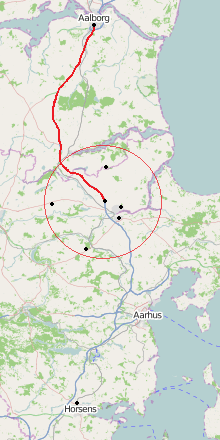
\includegraphics[scale=0.6]{images/AalborgtoHorsens1}  
  \end{center}
\end{frame}

\begin{frame}
  \frametitle{Experiments: The Naive Algorithm}
  \begin{center}
	  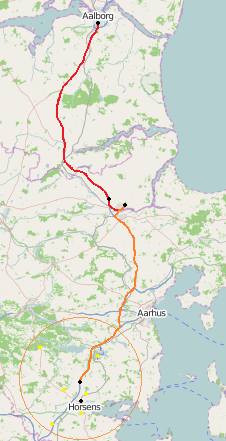
\includegraphics[scale=0.6]{images/AalborgtoHorsens2}  
  \end{center}
\end{frame}

\begin{frame}
  \frametitle{Experiments: The Naive Algorithm}
  \begin{center}
	  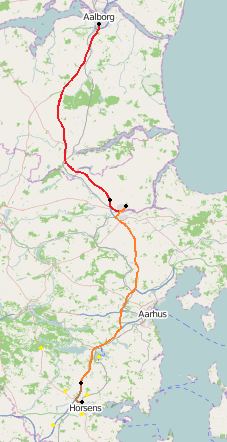
\includegraphics[scale=0.6]{images/AalborgtoHorsens3}  
  \end{center}
\end{frame}

\begin{frame}
  \frametitle{Experiments: Charge station density}
  \begin{center}
	  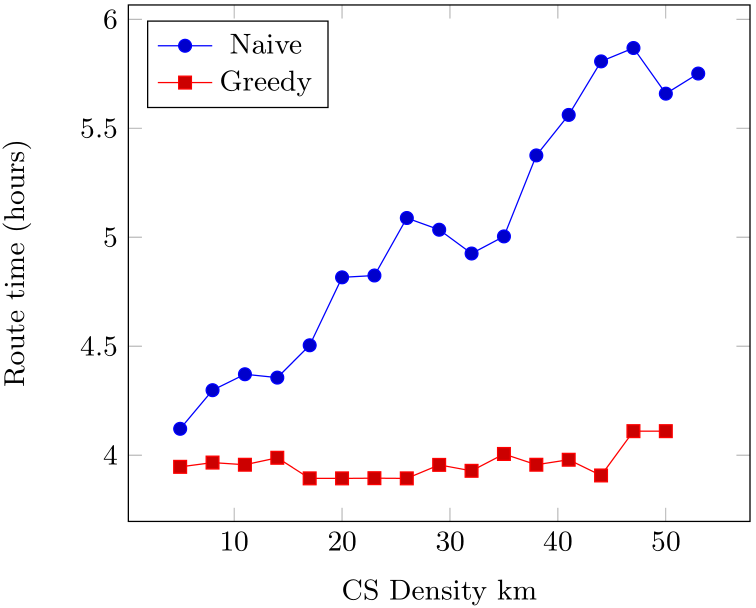
\includegraphics[scale=0.45]{images/CSdensity}  
  \end{center}
\end{frame}

\begin{frame}
  \frametitle{Experiments: Charge station density}
  \begin{columns}[c]
  \column{.5\textwidth} 
  	\begin{center}
  		\begin{figure}
	  	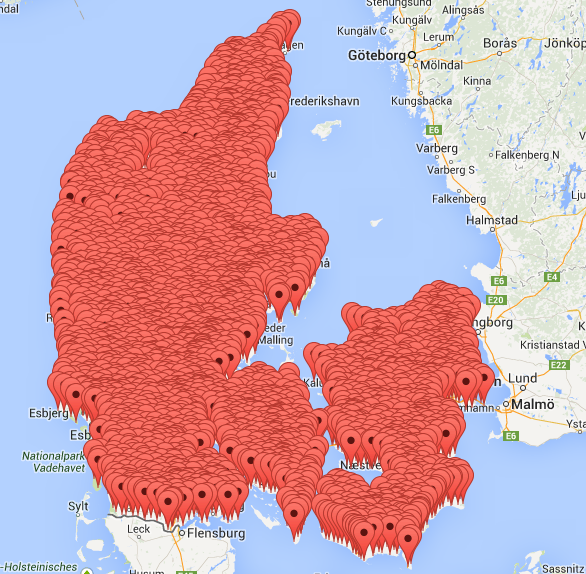
\includegraphics[scale=0.3]{images/density5km}
	  	\caption{5 km between Charge Stations}
	  	\end{figure} 
  	\end{center}
   \column{.5\textwidth}
   \begin{center}
   		\begin{figure}
	  	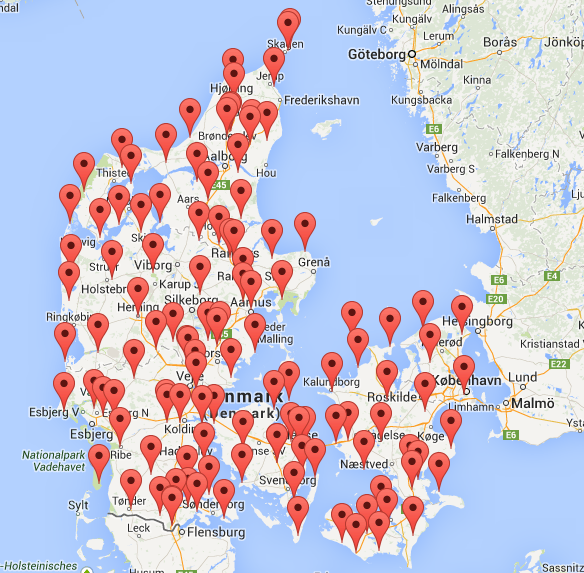
\includegraphics[scale=0.3]{images/density30km} 
	  	\caption{30 km between Charge Stations}
	  	\end{figure}
   \end{center}
   \end{columns} 
\end{frame}

\begin{frame}
  \frametitle{Experiments: Charge station density}
  \begin{center}
  	\begin{figure}
	  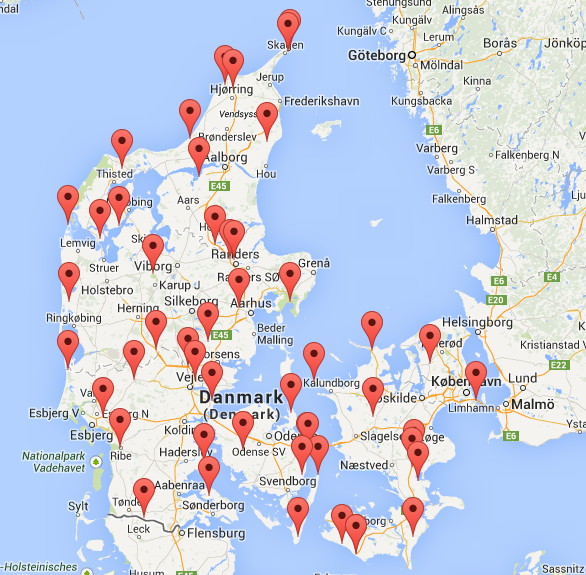
\includegraphics[scale=0.3]{images/density50km}  
	  \caption{50 km between Charge Stations}
	\end{figure}
  \end{center}
\end{frame}

\begin{frame}
  \frametitle{Experiments: Quality Assessment}
  \begin{itemize}
  	\item Standard setup
  	\item Average from 8 experiments
  \end{itemize}
  \vspace{0.8cm}
  {\large Results:}
  \begin{columns}[c]
    \column{.5\textwidth} 
    \begin{center}
    	\begin{tabular}{ | l l |}
    	\textcolor{blue}{Naive} & \textcolor{blue}{$7,461$} \\
    	\textcolor{red}{LP} & \textcolor{red}{$5,684$} \\
    	\end{tabular}
  	\end{center}
    \column{.5\textwidth}
    \begin{center}
    	\begin{tabular}{ | l l |}
    	\textcolor{blue}{Greedy} & \textcolor{blue}{$5,238$} \\
    	\textcolor{red}{LP} & \textcolor{red}{$5,228$} \\
    	\end{tabular}  
    \end{center}
   \end{columns} 
\end{frame}

\begin{frame}
  \frametitle{Conclusion}
  \begin{itemize}
  \item $0,1 \%$ worse than LP
  \item Not influenced much by CS density
  \item Too slow in practice
  \item Increasingly important
  \begin{itemize}
  \item Charging time significant
  \item Increasing EV sales
  \end{itemize}
  \end{itemize}
\end{frame}

\section{\scshape Future Work}
\subsection{Future Work}
\begin{frame}{Future Work}
\begin{itemize}
\item Variable Charge rates
\end{itemize}
\begin{figure}[h!]
  \centering
  Model S Charge Rate
    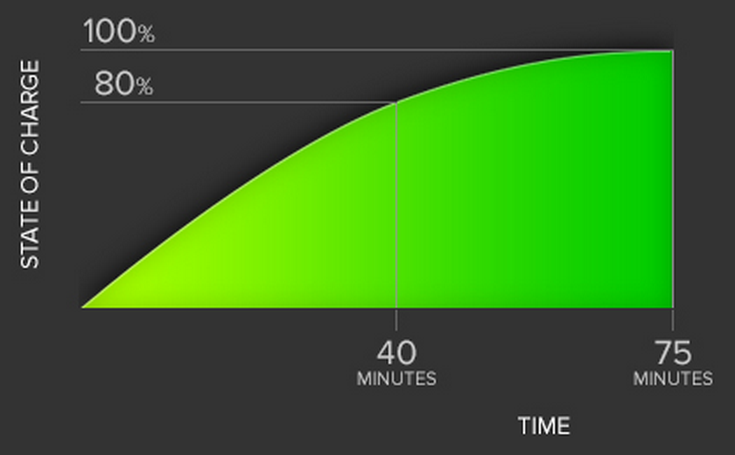
\includegraphics[width=0.7\textwidth]{images/chargerate}
  
      \tiny Credit: Tesla Motors, inc.
\end{figure}
\vspace{10cm}
\end{frame}

\begin{frame}{Future Work}
\begin{itemize}
\item Variable Charge rates
\item Better heuristic choices
\item Speed-up techniques
\item Branch \& Bound or some other pruning method
\end{itemize}
\vspace{10cm}
\end{frame}

\section{\scshape Q \& A}
%\subsection{Questions}
\begin{frame}{Q \& A time}
\end{frame}


\end{document}
